\begin{figure}[ht]
\centering
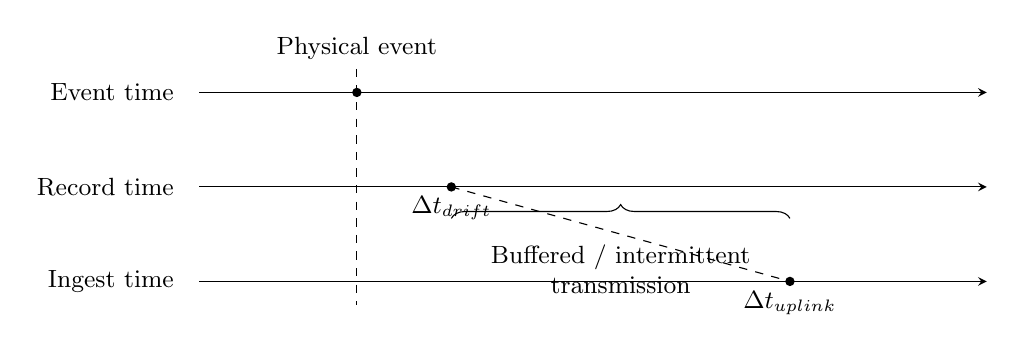
\begin{tikzpicture}[
  x=1cm,
  y=1cm,
  >=stealth,
  every node/.style={font=\small},
  timeline/.style={->},
  point/.style={circle,fill,inner sep=1.2pt}
]
  % Coordinates
  \def\xEvent{2}
  \def\xRecord{3.2}
  \def\xIngest{7.5}
  \def\xEnd{10}

  \coordinate (E) at (\xEvent,0);
  \coordinate (R) at (\xRecord,-1.2);
  \coordinate (I) at (\xIngest,-2.4);

  % Row labels
  \node[anchor=east] at (-0.2, 0) {Event time};
  \node[anchor=east] at (-0.2, -1.2) {Record time};
  \node[anchor=east] at (-0.2, -2.4) {Ingest time};

  % Timelines
  \draw[timeline] (0,0) -- (\xEnd,0);
  \draw[timeline] (0,-1.2) -- (\xEnd,-1.2);
  \draw[timeline] (0,-2.4) -- (\xEnd,-2.4);

  % Physical event marker
  \draw[dashed] (\xEvent,0.3) -- (\xEvent,-2.7);
  \node[anchor=south] at (\xEvent,0.3) {Physical event};

  % Points
  \node[point] at (E) {};
  \node[point] at (R) {};
  \node[point] at (I) {};

  % Drift and uplink offsets
  \draw[dashed] (\xEvent,-1.2) -- (R);
  \node[anchor=north] at (R) {$\Delta t_{\text{drift}}$};

  \draw[dashed] (R) -- (I);
  \node[anchor=north] at (I) {$\Delta t_{\text{uplink}}$};

  % Buffer annotation
  \draw[decorate,decoration={brace,amplitude=5pt}]
    (\xRecord,-1.6) -- (\xIngest,-1.6)
    node[midway,below=6pt,align=center,text width=4cm]{Buffered / intermittent\\ transmission};
\end{tikzpicture}
\caption{Temporal domains in a typical long-horizon sensing stack. A single physical event maps to divergent timestamps under clock drift and delayed uplink. Event time, record time, and ingest time must be represented explicitly to preserve causal coherence.}
\end{figure}